% Options for packages loaded elsewhere
\PassOptionsToPackage{unicode}{hyperref}
\PassOptionsToPackage{hyphens}{url}
%
\documentclass[
  9pt,
  ignorenonframetext,
]{beamer}
\usepackage{pgfpages}
\setbeamertemplate{caption}[numbered]
\setbeamertemplate{caption label separator}{: }
\setbeamercolor{caption name}{fg=normal text.fg}
\beamertemplatenavigationsymbolsempty
% Prevent slide breaks in the middle of a paragraph
\widowpenalties 1 10000
\raggedbottom
\setbeamertemplate{part page}{
  \centering
  \begin{beamercolorbox}[sep=16pt,center]{part title}
    \usebeamerfont{part title}\insertpart\par
  \end{beamercolorbox}
}
\setbeamertemplate{section page}{
  \centering
  \begin{beamercolorbox}[sep=12pt,center]{part title}
    \usebeamerfont{section title}\insertsection\par
  \end{beamercolorbox}
}
\setbeamertemplate{subsection page}{
  \centering
  \begin{beamercolorbox}[sep=8pt,center]{part title}
    \usebeamerfont{subsection title}\insertsubsection\par
  \end{beamercolorbox}
}
\AtBeginPart{
  \frame{\partpage}
}
\AtBeginSection{
  \ifbibliography
  \else
    \frame{\sectionpage}
  \fi
}
\AtBeginSubsection{
  \frame{\subsectionpage}
}
\usepackage{lmodern}
\usepackage{amssymb,amsmath}
\usepackage{ifxetex,ifluatex}
\ifnum 0\ifxetex 1\fi\ifluatex 1\fi=0 % if pdftex
  \usepackage[T1]{fontenc}
  \usepackage[utf8]{inputenc}
  \usepackage{textcomp} % provide euro and other symbols
\else % if luatex or xetex
  \usepackage{unicode-math}
  \defaultfontfeatures{Scale=MatchLowercase}
  \defaultfontfeatures[\rmfamily]{Ligatures=TeX,Scale=1}
\fi
\usetheme[]{Berkeley}
\usecolortheme{dove}
\usefonttheme{structurebold}
% Use upquote if available, for straight quotes in verbatim environments
\IfFileExists{upquote.sty}{\usepackage{upquote}}{}
\IfFileExists{microtype.sty}{% use microtype if available
  \usepackage[]{microtype}
  \UseMicrotypeSet[protrusion]{basicmath} % disable protrusion for tt fonts
}{}
\makeatletter
\@ifundefined{KOMAClassName}{% if non-KOMA class
  \IfFileExists{parskip.sty}{%
    \usepackage{parskip}
  }{% else
    \setlength{\parindent}{0pt}
    \setlength{\parskip}{6pt plus 2pt minus 1pt}}
}{% if KOMA class
  \KOMAoptions{parskip=half}}
\makeatother
\usepackage{xcolor}
\IfFileExists{xurl.sty}{\usepackage{xurl}}{} % add URL line breaks if available
\IfFileExists{bookmark.sty}{\usepackage{bookmark}}{\usepackage{hyperref}}
\hypersetup{
  pdftitle={Pesquisa reproduzível},
  pdfauthor={Frederico Bertholini},
  hidelinks,
  pdfcreator={LaTeX via pandoc}}
\urlstyle{same} % disable monospaced font for URLs
\newif\ifbibliography
\usepackage{color}
\usepackage{fancyvrb}
\newcommand{\VerbBar}{|}
\newcommand{\VERB}{\Verb[commandchars=\\\{\}]}
\DefineVerbatimEnvironment{Highlighting}{Verbatim}{commandchars=\\\{\}}
% Add ',fontsize=\small' for more characters per line
\usepackage{framed}
\definecolor{shadecolor}{RGB}{248,248,248}
\newenvironment{Shaded}{\begin{snugshade}}{\end{snugshade}}
\newcommand{\AlertTok}[1]{\textcolor[rgb]{0.94,0.16,0.16}{#1}}
\newcommand{\AnnotationTok}[1]{\textcolor[rgb]{0.56,0.35,0.01}{\textbf{\textit{#1}}}}
\newcommand{\AttributeTok}[1]{\textcolor[rgb]{0.77,0.63,0.00}{#1}}
\newcommand{\BaseNTok}[1]{\textcolor[rgb]{0.00,0.00,0.81}{#1}}
\newcommand{\BuiltInTok}[1]{#1}
\newcommand{\CharTok}[1]{\textcolor[rgb]{0.31,0.60,0.02}{#1}}
\newcommand{\CommentTok}[1]{\textcolor[rgb]{0.56,0.35,0.01}{\textit{#1}}}
\newcommand{\CommentVarTok}[1]{\textcolor[rgb]{0.56,0.35,0.01}{\textbf{\textit{#1}}}}
\newcommand{\ConstantTok}[1]{\textcolor[rgb]{0.00,0.00,0.00}{#1}}
\newcommand{\ControlFlowTok}[1]{\textcolor[rgb]{0.13,0.29,0.53}{\textbf{#1}}}
\newcommand{\DataTypeTok}[1]{\textcolor[rgb]{0.13,0.29,0.53}{#1}}
\newcommand{\DecValTok}[1]{\textcolor[rgb]{0.00,0.00,0.81}{#1}}
\newcommand{\DocumentationTok}[1]{\textcolor[rgb]{0.56,0.35,0.01}{\textbf{\textit{#1}}}}
\newcommand{\ErrorTok}[1]{\textcolor[rgb]{0.64,0.00,0.00}{\textbf{#1}}}
\newcommand{\ExtensionTok}[1]{#1}
\newcommand{\FloatTok}[1]{\textcolor[rgb]{0.00,0.00,0.81}{#1}}
\newcommand{\FunctionTok}[1]{\textcolor[rgb]{0.00,0.00,0.00}{#1}}
\newcommand{\ImportTok}[1]{#1}
\newcommand{\InformationTok}[1]{\textcolor[rgb]{0.56,0.35,0.01}{\textbf{\textit{#1}}}}
\newcommand{\KeywordTok}[1]{\textcolor[rgb]{0.13,0.29,0.53}{\textbf{#1}}}
\newcommand{\NormalTok}[1]{#1}
\newcommand{\OperatorTok}[1]{\textcolor[rgb]{0.81,0.36,0.00}{\textbf{#1}}}
\newcommand{\OtherTok}[1]{\textcolor[rgb]{0.56,0.35,0.01}{#1}}
\newcommand{\PreprocessorTok}[1]{\textcolor[rgb]{0.56,0.35,0.01}{\textit{#1}}}
\newcommand{\RegionMarkerTok}[1]{#1}
\newcommand{\SpecialCharTok}[1]{\textcolor[rgb]{0.00,0.00,0.00}{#1}}
\newcommand{\SpecialStringTok}[1]{\textcolor[rgb]{0.31,0.60,0.02}{#1}}
\newcommand{\StringTok}[1]{\textcolor[rgb]{0.31,0.60,0.02}{#1}}
\newcommand{\VariableTok}[1]{\textcolor[rgb]{0.00,0.00,0.00}{#1}}
\newcommand{\VerbatimStringTok}[1]{\textcolor[rgb]{0.31,0.60,0.02}{#1}}
\newcommand{\WarningTok}[1]{\textcolor[rgb]{0.56,0.35,0.01}{\textbf{\textit{#1}}}}
\setlength{\emergencystretch}{3em} % prevent overfull lines
\providecommand{\tightlist}{%
  \setlength{\itemsep}{0pt}\setlength{\parskip}{0pt}}
\setcounter{secnumdepth}{5}

\title{Pesquisa reproduzível}
\subtitle{Métodos Quantitativos Aplicados à Ciência Política}
\author{Frederico Bertholini}
\date{05.out.2020}

\begin{document}
\frame{\titlepage}

\begin{frame}[allowframebreaks]
  \tableofcontents[hideallsubsections]
\end{frame}
\hypertarget{nunca-esqueuxe7a}{%
\section{Nunca esqueça}\label{nunca-esqueuxe7a}}

\begin{frame}[fragile]{Pacotes e diretório de trabalho}
\protect\hypertarget{pacotes-e-diretuxf3rio-de-trabalho}{}
\begin{Shaded}
\begin{Highlighting}[]
\NormalTok{lista.de.pacotes =}\StringTok{ }\KeywordTok{c}\NormalTok{(}\StringTok{"tidyverse"}\NormalTok{,}\StringTok{"haven"}\NormalTok{,}\StringTok{"lubridate"}\NormalTok{,}
                     \StringTok{"janitor"}\NormalTok{,}\StringTok{"readxl"}\NormalTok{,}
                     \StringTok{"stringr"}\NormalTok{, }\StringTok{"magrittr"}\NormalTok{) }
                     \CommentTok{\# escreva a lista de pacotes}

\NormalTok{novos.pacotes \textless{}{-}}\StringTok{ }
\StringTok{  }\NormalTok{lista.de.pacotes[}\OperatorTok{!}\NormalTok{(lista.de.pacotes }\OperatorTok{\%in\%}
\StringTok{                      }\KeywordTok{installed.packages}\NormalTok{()[,}\StringTok{"Package"}\NormalTok{])]}

\ControlFlowTok{if}\NormalTok{(}\KeywordTok{length}\NormalTok{(novos.pacotes) }\OperatorTok{\textgreater{}}\StringTok{ }\DecValTok{0}\NormalTok{) \{}\KeywordTok{install.packages}\NormalTok{(novos.pacotes)\}}

\KeywordTok{lapply}\NormalTok{(lista.de.pacotes, require, }\DataTypeTok{character.only=}\NormalTok{T)}
\CommentTok{\#rm(lista.de.pacotes,novos.pacotes)}

\KeywordTok{rm}\NormalTok{(}\DataTypeTok{list =} \KeywordTok{ls}\NormalTok{())}
\KeywordTok{gc}\NormalTok{()}



\CommentTok{\# Definindo o diretorio de trabalho como do arquivo local}
\KeywordTok{setwd}\NormalTok{(}\KeywordTok{dirname}\NormalTok{(rstudioapi}\OperatorTok{::}\KeywordTok{getActiveDocumentContext}\NormalTok{()}\OperatorTok{$}\NormalTok{path))}

\KeywordTok{setwd}\NormalTok{(}\StringTok{"/Volumes/Macintosh HD/MQCP\_IPOL\_2020/Slides/aula 04"}\NormalTok{) }\CommentTok{\# mmudando meu direto}
\end{Highlighting}
\end{Shaded}
\end{frame}

\hypertarget{o-universo-tidyverse}{%
\section{O Universo tidyverse}\label{o-universo-tidyverse}}

\begin{frame}{Manifesto tidyverse}
\protect\hypertarget{manifesto-tidyverse}{}
\begin{itemize}
\item
  Reutilizar estruturas de dados existentes.
\item
  Organizar funções simples usando o pipe.
\item
  Aderir à programação funcional.
\item
  Projetado para ser usado por seres humanos.
\end{itemize}
\end{frame}

\begin{frame}{Manifesto tidy}
\protect\hypertarget{manifesto-tidy}{}
\begin{itemize}
\item
  Tidy Tools Manifesto
  \url{https://cran.r-project.org/web/packages/tidyverse/vignettes/manifesto.html}
\item
  Tidy data vignette
  \url{https://cran.r-project.org/web/packages/tidyr/vignettes/tidy-data.html}
\item
  Tidy Data paper \url{http://vita.had.co.nz/papers/tidy-data.pdf}
\item
  Conjunto de pacotes \url{https://www.tidyverse.org/packages/}
\end{itemize}
\end{frame}

\begin{frame}[fragile]{Conjunto de dados}
\protect\hypertarget{conjunto-de-dados}{}
Vamos trabalhar com a base \texttt{decisoes}, que contém decisões do
Tribunal de Justiça de São Paulo

\begin{Shaded}
\begin{Highlighting}[]
\NormalTok{decisoes \textless{}{-}}\StringTok{ }\KeywordTok{read\_rds}\NormalTok{(}\StringTok{"dados/decisoes.rds"}\NormalTok{) }\OperatorTok{\%\textgreater{}\%}
\StringTok{  }\NormalTok{janitor}\OperatorTok{::}\KeywordTok{clean\_names}\NormalTok{() }\CommentTok{\# com dois pontos eu não preciso usar library}
\KeywordTok{glimpse}\NormalTok{(decisoes)}
\end{Highlighting}
\end{Shaded}

\begin{verbatim}
## Rows: 11,731
## Columns: 9
## $ id_decisao     <chr> "11094999", "11093733", "11093677", "11093270", "110...
## $ n_processo     <chr> "0057003-20.2017.8.26.0000", "0052762-03.2017.8.26.0...
## $ classe_assunto <chr> "Habeas Corpus / Homicídio Simples", "Habeas Corpus ...
## $ municipio      <chr> "Cosmópolis", "São Paulo", "Ribeirão Preto", "Araçat...
## $ camara         <chr> "3ª Câmara de Direito Criminal", "3ª Câmara de Direi...
## $ data_decisao   <chr> "19/12/2017", "19/12/2017", "19/12/2017", "14/12/201...
## $ data_registro  <chr> "19/12/2017", "19/12/2017", "19/12/2017", "19/12/201...
## $ juiz           <chr> "Luiz Antonio Cardoso", "Luiz Antonio Cardoso", "Lui...
## $ txt_decisao    <chr> NA, NA, NA, "Execução Penal –  Comutação de Penas – ...
\end{verbatim}
\end{frame}

\begin{frame}[fragile]{Características do \texttt{dplyr}}
\protect\hypertarget{caracteruxedsticas-do-dplyr}{}
\begin{itemize}
\item
  A utilização é facilitada com o emprego do operador
  \texttt{\%\textgreater{}\%}
\item
  No primeiro argumento colocamos o \texttt{data.frame} ou o
  \texttt{tibble}, e nos outros argumentos colocamos o que queremos
  fazer.
\end{itemize}
\end{frame}

\begin{frame}[fragile]{As cinco funções principais do \texttt{dplyr}}
\protect\hypertarget{as-cinco-funuxe7uxf5es-principais-do-dplyr}{}
\begin{itemize}
\item
  \texttt{select}: selecionar colunas
\item
  \texttt{filter}: filtrar linhas
\item
  \texttt{mutate}: criar colunas
\item
  \texttt{summarise}: sumarizar colunas
\item
  \texttt{arrange}: ordenar linhas
\end{itemize}
\end{frame}

\hypertarget{tydyr}{%
\section{tydyr}\label{tydyr}}

\begin{frame}[fragile]{Alterando o formato de dados}
\protect\hypertarget{alterando-o-formato-de-dados}{}
Até agora, estudamos os principais ferramentas de transformação de dados
do \texttt{dplyr}. Agora vamos aumentar nossa caixa-de-ferramentas com
\texttt{tidyr}

\begin{itemize}
\tightlist
\item
  Carregando uma nova base de dados, que completa a de decisões.
\end{itemize}

\begin{Shaded}
\begin{Highlighting}[]
\NormalTok{processos \textless{}{-}}\StringTok{ }\KeywordTok{read\_rds}\NormalTok{(}\StringTok{"dados/processos\_nested.rds"}\NormalTok{)}
\end{Highlighting}
\end{Shaded}
\end{frame}

\begin{frame}{Fomato tidy}
\protect\hypertarget{fomato-tidy}{}
\begin{itemize}
\tightlist
\item
  Hadley Wickham \url{http://r4ds.had.co.nz/tidy-data.html}
\end{itemize}
\end{frame}

\begin{frame}[fragile]{Funções do pacote}
\protect\hypertarget{funuxe7uxf5es-do-pacote}{}
\begin{itemize}
\item
  Enquanto o \texttt{dplyr} faz recortes na base (com \texttt{filter()}e
  \texttt{select()}) e adições simples (\texttt{mutate()},
  \texttt{summarise()}), o \texttt{tidyr} mexe no \textbf{formato} da
  tabela (\texttt{gather()}, \texttt{spread()}) e faz modificações menos
  triviais.
\item
  As funções do \texttt{tidyr} geralmente vêm em pares com seus
  inversos:

  \begin{itemize}
  \tightlist
  \item
    \texttt{gather()} e \texttt{spread()}, -\textgreater{} substituídas
    por \texttt{pivot\_longer} e \texttt{pivot\_wider}
  \item
    \texttt{nest()} e \texttt{unnest()},
  \item
    \texttt{separate()} e \texttt{unite()}
  \end{itemize}
\end{itemize}
\end{frame}

\begin{frame}{Onde estamos}
\protect\hypertarget{onde-estamos}{}
\url{http://r4ds.had.co.nz/wrangle-intro.html}
\end{frame}

\begin{frame}[fragile]{\texttt{gather()}}
\protect\hypertarget{gather}{}
\begin{itemize}
\item
  \texttt{gather()} empilha o banco de dados
\item
  \texttt{pivot\_longer} empilha de um jeito ainda mais fácil
\end{itemize}

\begin{Shaded}
\begin{Highlighting}[]
\NormalTok{decisoes }\OperatorTok{\%\textgreater{}\%}\StringTok{ }
\StringTok{  }\KeywordTok{filter}\NormalTok{(}\OperatorTok{!}\KeywordTok{is.na}\NormalTok{(id\_decisao)) }\OperatorTok{\%\textgreater{}\%}\StringTok{ }
\StringTok{  }\KeywordTok{select}\NormalTok{(id\_decisao}\OperatorTok{:}\NormalTok{data\_registro) }\OperatorTok{\%\textgreater{}\%}\StringTok{ }
\StringTok{  }\CommentTok{\# 1. nome da coluna que vai guardar os nomes de colunas empilhadas}
\StringTok{  }\CommentTok{\# 2. nome da coluna que vai guardar os valores das colunas}
\StringTok{  }\CommentTok{\# 3. seleção das colunas a serem empilhadas}
\StringTok{  }\KeywordTok{gather}\NormalTok{(}\DataTypeTok{key=}\StringTok{"variavel"}\NormalTok{, }\DataTypeTok{value=}\StringTok{"valor"}\NormalTok{, }\OperatorTok{{-}}\NormalTok{id\_decisao) }\OperatorTok{\%\textgreater{}\%}\StringTok{ }
\StringTok{  }\KeywordTok{arrange}\NormalTok{(id\_decisao)}
\end{Highlighting}
\end{Shaded}

\begin{verbatim}
## # A tibble: 69,996 x 3
##    id_decisao variavel       valor                                        
##    <chr>      <chr>          <chr>                                        
##  1 11026431   n_processo     0000009-51.2015.8.26.0546                    
##  2 11026431   classe_assunto Apelação / Tráfico de Drogas e Condutas Afins
##  3 11026431   municipio      Itapira                                      
##  4 11026431   camara         5ª Câmara de Direito Criminal                
##  5 11026431   data_decisao   30/11/2017                                   
##  6 11026431   data_registro  01/12/2017                                   
##  7 11026432   n_processo     0002267-69.2013.8.26.0654                    
##  8 11026432   classe_assunto Apelação / Furto Qualificado                 
##  9 11026432   municipio      Vargem Grande Paulista                       
## 10 11026432   camara         5ª Câmara de Direito Criminal                
## # ... with 69,986 more rows
\end{verbatim}
\end{frame}

\begin{frame}[fragile]{\texttt{pivot\_longer}}
\protect\hypertarget{pivot_longer}{}
Base \texttt{relig\_income} do \texttt{tidyr} 3 variáveis:

\begin{itemize}
\tightlist
\item
  religion, nas linhas
\item
  income, nas colunas e
\item
  count, nas células
\end{itemize}

\begin{Shaded}
\begin{Highlighting}[]
\NormalTok{tidyr}\OperatorTok{::}\NormalTok{relig\_income}
\end{Highlighting}
\end{Shaded}

\begin{verbatim}
## # A tibble: 18 x 11
##    religion `<$10k` `$10-20k` `$20-30k` `$30-40k` `$40-50k` `$50-75k` `$75-100k`
##    <chr>      <dbl>     <dbl>     <dbl>     <dbl>     <dbl>     <dbl>      <dbl>
##  1 Agnostic      27        34        60        81        76       137        122
##  2 Atheist       12        27        37        52        35        70         73
##  3 Buddhist      27        21        30        34        33        58         62
##  4 Catholic     418       617       732       670       638      1116        949
##  5 Don’t k~      15        14        15        11        10        35         21
##  6 Evangel~     575       869      1064       982       881      1486        949
##  7 Hindu          1         9         7         9        11        34         47
##  8 Histori~     228       244       236       238       197       223        131
##  9 Jehovah~      20        27        24        24        21        30         15
## 10 Jewish        19        19        25        25        30        95         69
## 11 Mainlin~     289       495       619       655       651      1107        939
## 12 Mormon        29        40        48        51        56       112         85
## 13 Muslim         6         7         9        10         9        23         16
## 14 Orthodox      13        17        23        32        32        47         38
## 15 Other C~       9         7        11        13        13        14         18
## 16 Other F~      20        33        40        46        49        63         46
## 17 Other W~       5         2         3         4         2         7          3
## 18 Unaffil~     217       299       374       365       341       528        407
## # ... with 3 more variables: `$100-150k` <dbl>, `>150k` <dbl>, `Don't
## #   know/refused` <dbl>
\end{verbatim}
\end{frame}

\begin{frame}[fragile]{}
\protect\hypertarget{section}{}
\begin{Shaded}
\begin{Highlighting}[]
\NormalTok{tidyr}\OperatorTok{::}\NormalTok{relig\_income }\OperatorTok{\%\textgreater{}\%}
\StringTok{  }\KeywordTok{pivot\_longer}\NormalTok{(}\OperatorTok{!}\NormalTok{religion, }
               \DataTypeTok{names\_to =} \StringTok{"income"}\NormalTok{, }\CommentTok{\# diz a varável onde entrarão os nomes}
               \DataTypeTok{values\_to =} \StringTok{"count"} \CommentTok{\# diz a variável onde entrarão os valores}
\NormalTok{               )}
\end{Highlighting}
\end{Shaded}

\begin{verbatim}
## # A tibble: 180 x 3
##    religion income             count
##    <chr>    <chr>              <dbl>
##  1 Agnostic <$10k                 27
##  2 Agnostic $10-20k               34
##  3 Agnostic $20-30k               60
##  4 Agnostic $30-40k               81
##  5 Agnostic $40-50k               76
##  6 Agnostic $50-75k              137
##  7 Agnostic $75-100k             122
##  8 Agnostic $100-150k            109
##  9 Agnostic >150k                 84
## 10 Agnostic Don't know/refused    96
## # ... with 170 more rows
\end{verbatim}
\end{frame}

\begin{frame}[fragile]{\texttt{spread()}}
\protect\hypertarget{spread}{}
\begin{itemize}
\item
  \texttt{spread()} espalha uma variável nas colunas e preenche com
  outra variável
\item
  Função inversa de \texttt{gather}
\item
  Bem mais fácil com \texttt{pivot\_wider}
\end{itemize}

\begin{Shaded}
\begin{Highlighting}[]
\NormalTok{decisoes }\OperatorTok{\%\textgreater{}\%}\StringTok{ }
\StringTok{  }\KeywordTok{filter}\NormalTok{(}\OperatorTok{!}\KeywordTok{is.na}\NormalTok{(id\_decisao)) }\OperatorTok{\%\textgreater{}\%}\StringTok{ }
\StringTok{  }\KeywordTok{select}\NormalTok{(id\_decisao}\OperatorTok{:}\NormalTok{data\_registro) }\OperatorTok{\%\textgreater{}\%}\StringTok{ }
\StringTok{  }\KeywordTok{gather}\NormalTok{(key, value, }\OperatorTok{{-}}\NormalTok{id\_decisao) }\OperatorTok{\%\textgreater{}\%}\StringTok{ }
\StringTok{  }\CommentTok{\# 1. coluna a ser espalhada}
\StringTok{  }\CommentTok{\# 2. valores da coluna}
\StringTok{  }\KeywordTok{spread}\NormalTok{(key, value)}
\end{Highlighting}
\end{Shaded}

\begin{verbatim}
## # A tibble: 11,666 x 7
##    id_decisao camara classe_assunto data_decisao data_registro municipio
##    <chr>      <chr>  <chr>          <chr>        <chr>         <chr>    
##  1 11026431   5ª Câ~ Apelação / Tr~ 30/11/2017   01/12/2017    Itapira  
##  2 11026432   5ª Câ~ Apelação / Fu~ 30/11/2017   01/12/2017    Vargem G~
##  3 11026433   5ª Câ~ Apelação / Ro~ 30/11/2017   01/12/2017    Sertãozi~
##  4 11026434   12ª C~ Agravo de Exe~ 18/10/2017   01/12/2017    Ribeirão~
##  5 11026435   15ª C~ Apelação / Tr~ 30/11/2017   01/12/2017    São Paulo
##  6 11026442   5ª Câ~ Apelação / Es~ 30/11/2017   01/12/2017    Jales    
##  7 11026445   13ª C~ Apelação / Us~ 30/11/2017   01/12/2017    Santa Fé~
##  8 11026453   5ª Câ~ Apelação / Cr~ 30/11/2017   01/12/2017    Franca   
##  9 11026455   12ª C~ Apelação / Ro~ 05/07/2017   01/12/2017    Franca   
## 10 11026456   12ª C~ Apelação / Ro~ 03/05/2017   01/12/2017    São José~
## # ... with 11,656 more rows, and 1 more variable: n_processo <chr>
\end{verbatim}
\end{frame}

\begin{frame}[fragile]{\texttt{pivot\_wider}}
\protect\hypertarget{pivot_wider}{}
\begin{Shaded}
\begin{Highlighting}[]
\NormalTok{decisoes }\OperatorTok{\%\textgreater{}\%}\StringTok{ }
\StringTok{  }\KeywordTok{filter}\NormalTok{(}\OperatorTok{!}\KeywordTok{is.na}\NormalTok{(id\_decisao)) }\OperatorTok{\%\textgreater{}\%}\StringTok{ }
\StringTok{  }\KeywordTok{select}\NormalTok{(id\_decisao}\OperatorTok{:}\NormalTok{data\_registro) }\OperatorTok{\%\textgreater{}\%}\StringTok{ }
\StringTok{  }\KeywordTok{pivot\_longer}\NormalTok{(}\OperatorTok{!}\NormalTok{id\_decisao, }
               \DataTypeTok{names\_to =} \StringTok{"tipo"}\NormalTok{, }\CommentTok{\# diz a varável onde entrarão os nomes}
               \DataTypeTok{values\_to =} \StringTok{"info"} \CommentTok{\# diz a variável onde entrarão os valores}
\NormalTok{               ) }\OperatorTok{\%\textgreater{}\%}\StringTok{ }
\StringTok{  }\CommentTok{\# 1. coluna a ser espalhada}
\StringTok{  }\CommentTok{\# 2. valores da coluna}
\StringTok{  }\KeywordTok{pivot\_wider}\NormalTok{(}\DataTypeTok{names\_from =} \StringTok{"tipo"}\NormalTok{,}
              \DataTypeTok{values\_from =} \StringTok{"info"}\NormalTok{)}
\end{Highlighting}
\end{Shaded}

\begin{verbatim}
## # A tibble: 11,666 x 7
##    id_decisao n_processo classe_assunto municipio camara data_decisao
##    <chr>      <chr>      <chr>          <chr>     <chr>  <chr>       
##  1 11094999   0057003-2~ Habeas Corpus~ Cosmópol~ 3ª Câ~ 19/12/2017  
##  2 11093733   0052762-0~ Habeas Corpus~ São Paulo 3ª Câ~ 19/12/2017  
##  3 11093677   0055169-7~ Habeas Corpus~ Ribeirão~ 3ª Câ~ 19/12/2017  
##  4 11093270   9000580-8~ Agravo de Exe~ Araçatuba 8ª Câ~ 14/12/2017  
##  5 11093374   0052938-7~ Mandado de Se~ São Paulo 8ª Câ~ 14/12/2017  
##  6 11093320   9000723-7~ Agravo de Exe~ Presiden~ 8ª Câ~ 14/12/2017  
##  7 11091506   0003276-8~ Apelação / Tr~ Bertioga  8ª Câ~ 14/12/2017  
##  8 11093326   9000298-1~ Agravo de Exe~ Taubaté   8ª Câ~ 14/12/2017  
##  9 11092475   0004653-3~ Apelação / Tr~ Aparecida 8ª Câ~ 14/12/2017  
## 10 11093773   2221930-6~ Habeas Corpus~ Jandira   3ª Câ~ 19/12/2017  
## # ... with 11,656 more rows, and 1 more variable: data_registro <chr>
\end{verbatim}
\end{frame}

\begin{frame}[fragile]{}
\protect\hypertarget{section-1}{}
\begin{itemize}
\tightlist
\item
  Qual juiz julga a maior proporção de processos que tratam de drogas
\end{itemize}

-- Dica: construa um \texttt{data.frame} contendo as colunas juiz,
n\_processos\_drogas, n\_processos\_n\_drogas e total\_processos,
remodelando os dados para haver um juiz por linha e utilizando
\texttt{spread()}
\end{frame}

\begin{frame}[fragile]{Resolução}
\protect\hypertarget{resoluuxe7uxe3o}{}
\begin{verbatim}
## `summarise()` regrouping output by 'juiz' (override with `.groups` argument)
\end{verbatim}

\begin{verbatim}
## # A tibble: 65 x 5
## # Groups:   juiz [65]
##    juiz                            droga n_droga total proporcao
##    <chr>                           <dbl>   <dbl> <dbl>     <dbl>
##  1 Ivana David                        57     101   158     0.361
##  2 Diniz Fernando                     66     132   198     0.333
##  3 Sérgio Ribas                        1       2     3     0.333
##  4 Cesar Augusto Andrade de Castro    25      52    77     0.325
##  5 Paulo Rossi                        20      43    63     0.317
##  6 Sérgio Mazina Martins              54     117   171     0.316
##  7 Andrade Sampaio                    35      79   114     0.307
##  8 Moreira da Silva                   29      67    96     0.302
##  9 Machado de Andrade                  3       7    10     0.3  
## 10 Silmar Fernandes                   44     104   148     0.297
## # ... with 55 more rows
\end{verbatim}
\end{frame}

\begin{frame}[fragile]{}
\protect\hypertarget{section-2}{}
\begin{itemize}
\item
  Qual quantidade mensal de decisões por juiz?
\item
  Dica: use \texttt{data\_decisao} \texttt{dmy()} e \texttt{month()}
\end{itemize}
\end{frame}

\begin{frame}[fragile]{}
\protect\hypertarget{section-3}{}
\begin{Shaded}
\begin{Highlighting}[]
\NormalTok{decisoes }\OperatorTok{\%\textgreater{}\%}\StringTok{ }
\StringTok{  }\KeywordTok{filter}\NormalTok{(}\OperatorTok{!}\KeywordTok{is.na}\NormalTok{(txt\_decisao)) }\OperatorTok{\%\textgreater{}\%}
\StringTok{  }\KeywordTok{mutate}\NormalTok{(}\DataTypeTok{txt\_decisao =} \KeywordTok{tolower}\NormalTok{(txt\_decisao),}
         \DataTypeTok{droga =} \KeywordTok{str\_detect}\NormalTok{(txt\_decisao,}
    \StringTok{"droga|entorpecente|psicotr[óo]pico|maconha|haxixe|coca[íi]na"}\NormalTok{),}
    \DataTypeTok{droga=}\KeywordTok{case\_when}\NormalTok{(}
\NormalTok{      droga}\OperatorTok{==}\OtherTok{TRUE} \OperatorTok{\textasciitilde{}}\StringTok{ "droga"}\NormalTok{,}
\NormalTok{      droga}\OperatorTok{==}\OtherTok{FALSE} \OperatorTok{\textasciitilde{}}\StringTok{ "n\_droga"}
\NormalTok{    )) }\OperatorTok{\%\textgreater{}\%}
\StringTok{  }\KeywordTok{group\_by}\NormalTok{(juiz,droga) }\OperatorTok{\%\textgreater{}\%}
\StringTok{  }\KeywordTok{summarise}\NormalTok{(}\DataTypeTok{n=}\KeywordTok{n}\NormalTok{()) }\OperatorTok{\%\textgreater{}\%}
\StringTok{  }\KeywordTok{spread}\NormalTok{(droga,n,}\DataTypeTok{fill =} \DecValTok{0}\NormalTok{) }\OperatorTok{\%\textgreater{}\%}
\StringTok{  }\KeywordTok{mutate}\NormalTok{(}\DataTypeTok{total=}\NormalTok{droga}\OperatorTok{+}\NormalTok{n\_droga,}
         \DataTypeTok{proporcao=}\NormalTok{droga}\OperatorTok{/}\NormalTok{total)}
\end{Highlighting}
\end{Shaded}
\end{frame}

\begin{frame}[fragile]{Resultado}
\protect\hypertarget{resultado}{}
\begin{verbatim}
## `summarise()` regrouping output by 'juiz' (override with `.groups` argument)
\end{verbatim}

\begin{verbatim}
## # A tibble: 65 x 5
## # Groups:   juiz [65]
##    juiz                   droga n_droga total proporcao
##    <chr>                  <dbl>   <dbl> <dbl>     <dbl>
##  1 Airton Vieira             23     131   154     0.149
##  2 Alcides Malossi Junior    23      72    95     0.242
##  3 Alexandre Almeida         41     122   163     0.252
##  4 Amaro Thomé               36      96   132     0.273
##  5 Andrade Sampaio           35      79   114     0.307
##  6 Angélica de Almeida        2       6     8     0.25 
##  7 Antonio Tadeu Ottoni       0       1     1     0    
##  8 Bandeira Lins              0       2     2     0    
##  9 Camargo Aranha Filho      32     109   141     0.227
## 10 Camilo Léllis             32     133   165     0.194
## # ... with 55 more rows
\end{verbatim}
\end{frame}

\begin{frame}{Exemplo para o ggplot}
\protect\hypertarget{exemplo-para-o-ggplot}{}
\end{frame}

\begin{frame}[fragile]{Unindo e separando colunas}
\protect\hypertarget{unindo-e-separando-colunas}{}
\begin{itemize}
\tightlist
\item
  \texttt{unite} junta duas ou mais colunas usando algum separador
  (\texttt{\_}, por exemplo).
\item
  \texttt{separate} faz o inverso de \texttt{unite}, e uma coluna em
  várias usando um separador.
\end{itemize}
\end{frame}

\begin{frame}{Exemplo de separação de colunas}
\protect\hypertarget{exemplo-de-separauxe7uxe3o-de-colunas}{}
\begin{itemize}
\tightlist
\item
  Olhe os valores da variável classe\_assunto
\end{itemize}
\end{frame}

\begin{frame}[fragile]{Exemplo de separação de colunas}
\protect\hypertarget{exemplo-de-separauxe7uxe3o-de-colunas-1}{}
\begin{itemize}
\item
  Vamos separar a coluna classe\_assunto em duas colunas
\item
  coluna classe e coluna assunto
\item
  Existe separador? -\textgreater{} sim, \texttt{/}
\item
  Usei count apenas em assunto
\end{itemize}
\end{frame}

\begin{frame}[fragile]{Em ação}
\protect\hypertarget{em-auxe7uxe3o}{}
\begin{Shaded}
\begin{Highlighting}[]
\NormalTok{decisoes }\OperatorTok{\%\textgreater{}\%}\StringTok{ }
\StringTok{  }\KeywordTok{select}\NormalTok{(n\_processo, classe\_assunto) }\OperatorTok{\%\textgreater{}\%}\StringTok{ }
\StringTok{  }\KeywordTok{separate}\NormalTok{(classe\_assunto, }\KeywordTok{c}\NormalTok{(}\StringTok{\textquotesingle{}classe\textquotesingle{}}\NormalTok{, }\StringTok{\textquotesingle{}assunto\textquotesingle{}}\NormalTok{), }\DataTypeTok{sep =} \StringTok{\textquotesingle{} / \textquotesingle{}}\NormalTok{, }
           \DataTypeTok{extra =} \StringTok{\textquotesingle{}merge\textquotesingle{}}\NormalTok{, }\DataTypeTok{fill =} \StringTok{\textquotesingle{}right\textquotesingle{}}\NormalTok{) }\OperatorTok{\%\textgreater{}\%}\StringTok{ }
\StringTok{  }\KeywordTok{count}\NormalTok{(assunto, }\DataTypeTok{sort =} \OtherTok{TRUE}\NormalTok{)}

\CommentTok{\#\# count é um jeito resumido de usar group\_by() \%\textgreater{}\% summarise(n())}
\end{Highlighting}
\end{Shaded}
\end{frame}

\begin{frame}[fragile]{Em ação}
\protect\hypertarget{em-auxe7uxe3o-1}{}
\begin{verbatim}
## # A tibble: 152 x 2
##    assunto                                n
##    <chr>                              <int>
##  1 Tráfico de Drogas e Condutas Afins  2441
##  2 Pena Privativa de Liberdade         1106
##  3 Roubo Majorado                      1093
##  4 Furto Qualificado                    838
##  5 Roubo                                780
##  6 Progressão de Regime                 607
##  7 Furto                                450
##  8 Receptação                           353
##  9 Homicídio Qualificado                329
## 10 Crimes de Trânsito                   322
## # ... with 142 more rows
\end{verbatim}
\end{frame}

\begin{frame}[fragile]{List columns: \texttt{nest()} e
\texttt{unnest()}}
\protect\hypertarget{list-columns-nest-e-unnest}{}
\texttt{nest()} e \texttt{unnest()} são operações inversas e servem para
tratar dados complexos, como o que temos em \texttt{processos}

\begin{Shaded}
\begin{Highlighting}[]
\NormalTok{d\_partes \textless{}{-}}\StringTok{ }\NormalTok{processos }\OperatorTok{\%\textgreater{}\%}\StringTok{ }
\StringTok{  }\KeywordTok{select}\NormalTok{(n\_processo, partes) }\OperatorTok{\%\textgreater{}\%}\StringTok{ }
\StringTok{  }\KeywordTok{unnest}\NormalTok{(partes)}
\end{Highlighting}
\end{Shaded}
\end{frame}

\begin{frame}[fragile]{}
\protect\hypertarget{section-4}{}
As list columns são uma forma condensada de guardar dados que estariam
em múltiplas tabelas. Por exemplo, uma alternativa à colocar as
\texttt{partes} numa list column seria guardar a tabela
\texttt{d\_partes} separadamente.

\begin{Shaded}
\begin{Highlighting}[]
\KeywordTok{glimpse}\NormalTok{(d\_partes)}
\end{Highlighting}
\end{Shaded}

\begin{verbatim}
## Rows: 37,579
## Columns: 5
## $ n_processo <chr> "0000003-71.2016.8.26.0073", "0000003-71.2016.8.26.0073"...
## $ id         <int> 1, 1, 2, 1, 1, 2, 1, 1, 2, 1, 1, 2, 1, 1, 2, 1, 1, 2, 1,...
## $ name       <chr> "JOSE MARIA JUSTINO NETO", "Defensoria Pública do Estado...
## $ part       <chr> "Apelante", "Apelante", "Apelado", "Apelante", "Apelante...
## $ role       <chr> "Apelante", "Apelante", "Apelado", "Apelante", "Advogado...
\end{verbatim}
\end{frame}

\begin{frame}[fragile]{Duplicatas}
\protect\hypertarget{duplicatas}{}
Para retirar duplicatas, utilizar \texttt{distinct}. Ele considera
apenas a primeira linha em que encontra um padrão para as combinações de
variáveis escolhidas e descarta as demais.

\begin{Shaded}
\begin{Highlighting}[]
\NormalTok{decisoes }\OperatorTok{\%\textgreater{}\%}\StringTok{ }
\StringTok{  }\KeywordTok{distinct}\NormalTok{(municipio)}
\end{Highlighting}
\end{Shaded}

\begin{verbatim}
## # A tibble: 315 x 1
##    municipio          
##    <chr>              
##  1 Cosmópolis         
##  2 São Paulo          
##  3 Ribeirão Preto     
##  4 Araçatuba          
##  5 Presidente Prudente
##  6 Bertioga           
##  7 Taubaté            
##  8 Aparecida          
##  9 Jandira            
## 10 Flórida Paulista   
## # ... with 305 more rows
\end{verbatim}
\end{frame}

\begin{frame}[fragile]{Por coluna}
\protect\hypertarget{por-coluna}{}
Para manter as demais colunas, use \texttt{.keep\_all=}:

\begin{Shaded}
\begin{Highlighting}[]
\NormalTok{decisoes }\OperatorTok{\%\textgreater{}\%}
\StringTok{  }\KeywordTok{distinct}\NormalTok{(municipio, camara, }
           \DataTypeTok{.keep\_all =} \OtherTok{TRUE}\NormalTok{)}
\end{Highlighting}
\end{Shaded}

\begin{verbatim}
## # A tibble: 2,760 x 9
##    id_decisao n_processo classe_assunto municipio camara data_decisao
##    <chr>      <chr>      <chr>          <chr>     <chr>  <chr>       
##  1 11094999   0057003-2~ Habeas Corpus~ Cosmópol~ 3ª Câ~ 19/12/2017  
##  2 11093733   0052762-0~ Habeas Corpus~ São Paulo 3ª Câ~ 19/12/2017  
##  3 11093677   0055169-7~ Habeas Corpus~ Ribeirão~ 3ª Câ~ 19/12/2017  
##  4 11093270   9000580-8~ Agravo de Exe~ Araçatuba 8ª Câ~ 14/12/2017  
##  5 11093374   0052938-7~ Mandado de Se~ São Paulo 8ª Câ~ 14/12/2017  
##  6 11093320   9000723-7~ Agravo de Exe~ Presiden~ 8ª Câ~ 14/12/2017  
##  7 11091506   0003276-8~ Apelação / Tr~ Bertioga  8ª Câ~ 14/12/2017  
##  8 11093326   9000298-1~ Agravo de Exe~ Taubaté   8ª Câ~ 14/12/2017  
##  9 11092475   0004653-3~ Apelação / Tr~ Aparecida 8ª Câ~ 14/12/2017  
## 10 11093773   2221930-6~ Habeas Corpus~ Jandira   3ª Câ~ 19/12/2017  
## # ... with 2,750 more rows, and 3 more variables: data_registro <chr>,
## #   juiz <chr>, txt_decisao <chr>
\end{verbatim}
\end{frame}

\begin{frame}[fragile]{\texttt{janitor::get\_dupes()}}
\protect\hypertarget{janitorget_dupes}{}
Use \texttt{janitor::get\_dupes()} para averiguar os casos em que há
repetição de combinações de colunas.

\begin{Shaded}
\begin{Highlighting}[]
\NormalTok{decisoes }\OperatorTok{\%\textgreater{}\%}\StringTok{ }
\StringTok{  }\KeywordTok{get\_dupes}\NormalTok{(n\_processo)}
\end{Highlighting}
\end{Shaded}

\begin{verbatim}
## # A tibble: 114 x 10
##    n_processo dupe_count id_decisao classe_assunto municipio camara data_decisao
##    <chr>           <int> <chr>      <chr>          <chr>     <chr>  <chr>       
##  1 0000276-8~          2 11051087   Apelação / Tr~ Itaporan~ 2ª Câ~ 27/11/2017  
##  2 0000276-8~          2 11093633   Embargos de D~ Itaporan~ 2ª Câ~ 18/12/2017  
##  3 0000358-1~          2 11108278   Embargos de D~ São Paulo 2ª Câ~ 15/01/2018  
##  4 0000358-1~          2 11028129   Apelação / Ro~ São Paulo 2ª Câ~ 27/11/2017  
##  5 0002236-1~          2 11041351   Apelação / Co~ Nhandeara 1ª Câ~ 27/11/2017  
##  6 0002236-1~          2 11041352   Apelação / Co~ Nhandeara 1ª Câ~ 27/11/2017  
##  7 0004453-2~          2 11041132   Apelação / Tr~ São Paulo 2ª Câ~ 13/11/2017  
##  8 0004453-2~          2 11093635   Embargos de D~ São Paulo 2ª Câ~ 18/12/2017  
##  9 0004636-5~          3 11032094   Apelação / Tr~ Olímpia   2ª Câ~ 27/11/2017  
## 10 0004636-5~          3 11032093   Apelação / Tr~ Olímpia   2ª Câ~ 27/11/2017  
## # ... with 104 more rows, and 3 more variables: data_registro <chr>,
## #   juiz <chr>, txt_decisao <chr>
\end{verbatim}
\end{frame}

\hypertarget{joins}{%
\section{Joins}\label{joins}}

\begin{frame}{Dados relacionais}
\protect\hypertarget{dados-relacionais}{}
\begin{itemize}
\tightlist
\item
  Hadley Wickham \url{http://r4ds.had.co.nz/relational-data.html}
\end{itemize}
\end{frame}

\begin{frame}[fragile]{Principais funções}
\protect\hypertarget{principais-funuxe7uxf5es}{}
Para juntar tabelas, usar \texttt{inner\_join}, \texttt{left\_join},
\texttt{anti\_join}, etc.
\end{frame}

\begin{frame}{Visualizando}
\protect\hypertarget{visualizando}{}
\end{frame}

\begin{frame}[fragile]{Exemplo de inner join:}
\protect\hypertarget{exemplo-de-inner-join}{}
\begin{Shaded}
\begin{Highlighting}[]
\NormalTok{a \textless{}{-}}\StringTok{ }\NormalTok{decisoes }\OperatorTok{\%\textgreater{}\%}\StringTok{ }
\StringTok{  }\KeywordTok{filter}\NormalTok{(data\_registro }\OperatorTok{==}\StringTok{ "18/01/2018"}\NormalTok{, }\OperatorTok{!}\KeywordTok{is.na}\NormalTok{(id\_decisao)) }\OperatorTok{\%\textgreater{}\%}\StringTok{ }
\StringTok{  }\KeywordTok{select}\NormalTok{(id\_decisao, n\_processo) }\OperatorTok{\%\textgreater{}\%}\StringTok{ }
\StringTok{  }\KeywordTok{inner\_join}\NormalTok{(processos, }\StringTok{"n\_processo"}\NormalTok{)}
\end{Highlighting}
\end{Shaded}
\end{frame}

\begin{frame}[fragile]{}
\protect\hypertarget{section-5}{}
\begin{verbatim}
## # A tibble: 169 x 5
##    id_decisao n_processo             infos           partes        results      
##    <chr>      <chr>                  <list>          <list>        <list>       
##  1 11109089   0003779-93.2015.8.26.~ <tibble [14 x ~ <tibble [3 x~ <tibble [1 x~
##  2 11109088   3001293-25.2013.8.26.~ <tibble [13 x ~ <tibble [3 x~ <tibble [1 x~
##  3 11108246   0063566-45.2015.8.26.~ <tibble [14 x ~ <tibble [3 x~ <tibble [1 x~
##  4 11108245   0003528-84.2015.8.26.~ <tibble [14 x ~ <tibble [3 x~ <tibble [1 x~
##  5 11109087   0008470-76.2015.8.26.~ <tibble [14 x ~ <tibble [4 x~ <tibble [1 x~
##  6 11109086   0013767-62.2012.8.26.~ <tibble [14 x ~ <tibble [4 x~ <tibble [1 x~
##  7 11109085   3019561-54.2013.8.26.~ <tibble [14 x ~ <tibble [3 x~ <tibble [1 x~
##  8 11108348   0003072-91.2017.8.26.~ <tibble [11 x ~ <tibble [3 x~ <tibble [1 x~
##  9 11108725   0009578-41.2017.8.26.~ <tibble [12 x ~ <tibble [4 x~ <tibble [1 x~
## 10 11108347   3001116-52.2013.8.26.~ <tibble [12 x ~ <tibble [3 x~ <tibble [1 x~
## # ... with 159 more rows
\end{verbatim}
\end{frame}

\begin{frame}[fragile]{Exemplo de right join:}
\protect\hypertarget{exemplo-de-right-join}{}
\begin{Shaded}
\begin{Highlighting}[]
\NormalTok{b \textless{}{-}}\StringTok{ }\NormalTok{decisoes }\OperatorTok{\%\textgreater{}\%}\StringTok{ }
\StringTok{  }\KeywordTok{filter}\NormalTok{(data\_registro }\OperatorTok{==}\StringTok{ "18/01/2018"}\NormalTok{, }\OperatorTok{!}\KeywordTok{is.na}\NormalTok{(id\_decisao)) }\OperatorTok{\%\textgreater{}\%}\StringTok{ }
\StringTok{  }\KeywordTok{select}\NormalTok{(id\_decisao, n\_processo) }\OperatorTok{\%\textgreater{}\%}\StringTok{ }
\StringTok{  }\KeywordTok{right\_join}\NormalTok{(processos, }\StringTok{"n\_processo"}\NormalTok{)}
\end{Highlighting}
\end{Shaded}
\end{frame}

\begin{frame}[fragile]{}
\protect\hypertarget{section-6}{}
\begin{verbatim}
## # A tibble: 11,638 x 5
##    id_decisao n_processo             infos           partes        results      
##    <chr>      <chr>                  <list>          <list>        <list>       
##  1 11109089   0003779-93.2015.8.26.~ <tibble [14 x ~ <tibble [3 x~ <tibble [1 x~
##  2 11109088   3001293-25.2013.8.26.~ <tibble [13 x ~ <tibble [3 x~ <tibble [1 x~
##  3 11108246   0063566-45.2015.8.26.~ <tibble [14 x ~ <tibble [3 x~ <tibble [1 x~
##  4 11108245   0003528-84.2015.8.26.~ <tibble [14 x ~ <tibble [3 x~ <tibble [1 x~
##  5 11109087   0008470-76.2015.8.26.~ <tibble [14 x ~ <tibble [4 x~ <tibble [1 x~
##  6 11109086   0013767-62.2012.8.26.~ <tibble [14 x ~ <tibble [4 x~ <tibble [1 x~
##  7 11109085   3019561-54.2013.8.26.~ <tibble [14 x ~ <tibble [3 x~ <tibble [1 x~
##  8 11108348   0003072-91.2017.8.26.~ <tibble [11 x ~ <tibble [3 x~ <tibble [1 x~
##  9 11108725   0009578-41.2017.8.26.~ <tibble [12 x ~ <tibble [4 x~ <tibble [1 x~
## 10 11108347   3001116-52.2013.8.26.~ <tibble [12 x ~ <tibble [3 x~ <tibble [1 x~
## # ... with 11,628 more rows
\end{verbatim}
\end{frame}

\hypertarget{limpeza}{%
\section{Limpeza}\label{limpeza}}

\begin{frame}[fragile]{Duplicatas}
\protect\hypertarget{duplicatas-1}{}
Para retirar duplicatas, utilizar \texttt{distinct}. Ele considera
apenas a primeira linha em que encontra um padrão para as combinações de
variáveis escolhidas e descarta as demais.

\begin{Shaded}
\begin{Highlighting}[]
\NormalTok{decisoes }\OperatorTok{\%\textgreater{}\%}\StringTok{ }
\StringTok{  }\KeywordTok{distinct}\NormalTok{(municipio)}
\end{Highlighting}
\end{Shaded}
\end{frame}

\begin{frame}[fragile]{}
\protect\hypertarget{section-7}{}
\begin{verbatim}
## # A tibble: 315 x 1
##    municipio          
##    <chr>              
##  1 Cosmópolis         
##  2 São Paulo          
##  3 Ribeirão Preto     
##  4 Araçatuba          
##  5 Presidente Prudente
##  6 Bertioga           
##  7 Taubaté            
##  8 Aparecida          
##  9 Jandira            
## 10 Flórida Paulista   
## # ... with 305 more rows
\end{verbatim}
\end{frame}

\begin{frame}[fragile]{Por coluna}
\protect\hypertarget{por-coluna-1}{}
Para manter as demais colunas, use \texttt{.keep\_all=}:

\begin{Shaded}
\begin{Highlighting}[]
\NormalTok{decisoes }\OperatorTok{\%\textgreater{}\%}
\StringTok{  }\KeywordTok{distinct}\NormalTok{(municipio, camara, }
           \DataTypeTok{.keep\_all =} \OtherTok{TRUE}\NormalTok{)}
\end{Highlighting}
\end{Shaded}
\end{frame}

\begin{frame}[fragile]{}
\protect\hypertarget{section-8}{}
\begin{verbatim}
## # A tibble: 2,760 x 9
##    id_decisao n_processo classe_assunto municipio camara data_decisao
##    <chr>      <chr>      <chr>          <chr>     <chr>  <chr>       
##  1 11094999   0057003-2~ Habeas Corpus~ Cosmópol~ 3ª Câ~ 19/12/2017  
##  2 11093733   0052762-0~ Habeas Corpus~ São Paulo 3ª Câ~ 19/12/2017  
##  3 11093677   0055169-7~ Habeas Corpus~ Ribeirão~ 3ª Câ~ 19/12/2017  
##  4 11093270   9000580-8~ Agravo de Exe~ Araçatuba 8ª Câ~ 14/12/2017  
##  5 11093374   0052938-7~ Mandado de Se~ São Paulo 8ª Câ~ 14/12/2017  
##  6 11093320   9000723-7~ Agravo de Exe~ Presiden~ 8ª Câ~ 14/12/2017  
##  7 11091506   0003276-8~ Apelação / Tr~ Bertioga  8ª Câ~ 14/12/2017  
##  8 11093326   9000298-1~ Agravo de Exe~ Taubaté   8ª Câ~ 14/12/2017  
##  9 11092475   0004653-3~ Apelação / Tr~ Aparecida 8ª Câ~ 14/12/2017  
## 10 11093773   2221930-6~ Habeas Corpus~ Jandira   3ª Câ~ 19/12/2017  
## # ... with 2,750 more rows, and 3 more variables: data_registro <chr>,
## #   juiz <chr>, txt_decisao <chr>
\end{verbatim}
\end{frame}

\begin{frame}[fragile]{\texttt{janitor::get\_dupes()}}
\protect\hypertarget{janitorget_dupes-1}{}
Use \texttt{janitor::get\_dupes()} para averiguar os casos em que há
repetição de combinações de colunas.

\begin{Shaded}
\begin{Highlighting}[]
\NormalTok{decisoes }\OperatorTok{\%\textgreater{}\%}\StringTok{ }
\StringTok{  }\KeywordTok{get\_dupes}\NormalTok{(n\_processo)}
\end{Highlighting}
\end{Shaded}
\end{frame}

\begin{frame}[fragile]{}
\protect\hypertarget{section-9}{}
\begin{verbatim}
## # A tibble: 114 x 10
##    n_processo dupe_count id_decisao classe_assunto municipio camara data_decisao
##    <chr>           <int> <chr>      <chr>          <chr>     <chr>  <chr>       
##  1 0000276-8~          2 11051087   Apelação / Tr~ Itaporan~ 2ª Câ~ 27/11/2017  
##  2 0000276-8~          2 11093633   Embargos de D~ Itaporan~ 2ª Câ~ 18/12/2017  
##  3 0000358-1~          2 11108278   Embargos de D~ São Paulo 2ª Câ~ 15/01/2018  
##  4 0000358-1~          2 11028129   Apelação / Ro~ São Paulo 2ª Câ~ 27/11/2017  
##  5 0002236-1~          2 11041351   Apelação / Co~ Nhandeara 1ª Câ~ 27/11/2017  
##  6 0002236-1~          2 11041352   Apelação / Co~ Nhandeara 1ª Câ~ 27/11/2017  
##  7 0004453-2~          2 11041132   Apelação / Tr~ São Paulo 2ª Câ~ 13/11/2017  
##  8 0004453-2~          2 11093635   Embargos de D~ São Paulo 2ª Câ~ 18/12/2017  
##  9 0004636-5~          3 11032094   Apelação / Tr~ Olímpia   2ª Câ~ 27/11/2017  
## 10 0004636-5~          3 11032093   Apelação / Tr~ Olímpia   2ª Câ~ 27/11/2017  
## # ... with 104 more rows, and 3 more variables: data_registro <chr>,
## #   juiz <chr>, txt_decisao <chr>
\end{verbatim}
\end{frame}

\begin{frame}[fragile]{}
\protect\hypertarget{section-10}{}
\begin{itemize}
\item
  \href{http://sfirke.github.io/janitor/articles/janitor.html}{Janitor
  exemplos}
\item
  \href{https://www.analyticsvidhya.com/blog/2016/03/tutorial-powerful-packages-imputing-missing-values/}{Missing
  e imputação}
\item
  \href{https://amices.org/mice/}{mice}
\item
  Outliers (critérios, limpeza e gráficos)
\item
  \texttt{stringi} e \texttt{stringr}--\textgreater{} expressões
  regulares
\end{itemize}
\end{frame}

\hypertarget{pesquisa-reproduzuxedvel}{%
\section{Pesquisa reproduzível}\label{pesquisa-reproduzuxedvel}}

\begin{frame}{Por quê?}
\protect\hypertarget{por-quuxea}{}
\begin{itemize}
\item
  Pra ciência
\item
  Pra você
\end{itemize}
\end{frame}

\begin{frame}{Ferramentas}
\protect\hypertarget{ferramentas}{}
\begin{itemize}
\item
  R e RStudio (ok)
\item
  Github
\item
  knitr e rmarkdown
\item
  LaTeX
\end{itemize}
\end{frame}

\begin{frame}{Fluxo de trabalho}
\protect\hypertarget{fluxo-de-trabalho}{}
\begin{enumerate}
\item
  Coleta
\item
  Análise
\item
  Comunicação
\end{enumerate}
\end{frame}

\begin{frame}{}
\protect\hypertarget{section-11}{}
\begin{center}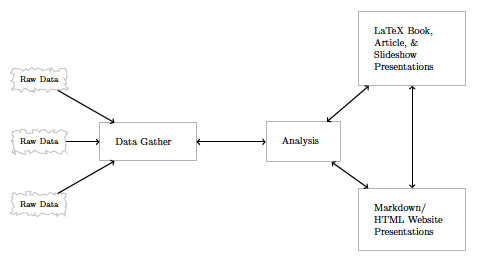
\includegraphics[width=1\linewidth]{imgs/fluxo_gandrud} \end{center}
\end{frame}

\begin{frame}{Dicas}
\protect\hypertarget{dicas}{}
\begin{enumerate}
\item
  Documente tudo!
\item
  Tudo é um arquivo (de texto).
\item
  Todos os arquivos devem ser legíveis (por humanos).
\item
  Relacione explicitamente seus arquivos.
\item
  Tenha um plano para organizar, armazenar e disponibilizar seus
  arquivos.
\end{enumerate}
\end{frame}

\hypertarget{versionando-projetos}{%
\section{Versionando projetos}\label{versionando-projetos}}

\begin{frame}{}
\protect\hypertarget{section-12}{}
\end{frame}

\begin{frame}{Repositório: Criação de repositório do projeto no Github}
\protect\hypertarget{reposituxf3rio-criauxe7uxe3o-de-reposituxf3rio-do-projeto-no-github}{}
\end{frame}

\begin{frame}{.Rproj: Criação do Projeto no RStudio}
\protect\hypertarget{rproj-criauxe7uxe3o-do-projeto-no-rstudio}{}
\end{frame}

\begin{frame}{Commit: Editando e ``Commitando'' as mudanças no código}
\protect\hypertarget{commit-editando-e-commitando-as-mudanuxe7as-no-cuxf3digo}{}
\end{frame}

\begin{frame}{Push: Subindo os commits para o Github}
\protect\hypertarget{push-subindo-os-commits-para-o-github}{}
\end{frame}

\begin{frame}{Pull: Baixando o estado atual do projeto}
\protect\hypertarget{pull-baixando-o-estado-atual-do-projeto}{}
\end{frame}

\hypertarget{ioslides-no-rmarkdown}{%
\section{ioslides no Rmarkdown}\label{ioslides-no-rmarkdown}}

\begin{frame}{Trabalhando com slides no RMarkdown}
\protect\hypertarget{trabalhando-com-slides-no-rmarkdown}{}
\begin{itemize}
\item
  Manual \url{https://rmarkdown.rstudio.com/lesson-11.html}
\item
  Galeria \url{https://rmarkdown.rstudio.com/gallery.html}
\end{itemize}

File ==\textgreater{} New file ==\textgreater{} R Markdown
==\textgreater{} Presentation

\begin{itemize}
\tightlist
\item
  HTML (ioslides)
\end{itemize}
\end{frame}

\begin{frame}[fragile]{Trabalhando no .rmd}
\protect\hypertarget{trabalhando-no-.rmd}{}
\begin{itemize}
\item
  Opções e detalhes do ioslides
  \url{https://rmarkdown.rstudio.com/ioslides_presentation_format\#overview}
\item
  Mais referências
  \url{https://bookdown.org/yihui/rmarkdown/ioslides-presentation.html}
\item
  Montando o arquivo \texttt{ìndex.rmd}
\end{itemize}
\end{frame}

\begin{frame}[fragile]{gh-pages}
\protect\hypertarget{gh-pages}{}
\begin{itemize}
\item
  novo ``branch''
\item
  nome \texttt{gh-pages}
\item
  arquivo \texttt{ìndex.html} precisa estar na raiz
\item
  a cada alteração de \texttt{ìndex.rmd} e \texttt{ìndex.html}, merge de
  master para gh-pages OU SIMPLESMENTE apague o branch e recrie o
  gh-pages
\item
  Suestão: só crie o branch gh-pages quando concluir seu trabalho e
  fizer o
\item
  Seu site estará no endereço ==\textgreater{}
  nome\_de\_usuario.github.io/nome\_do\_repositorio/
\item
  ATENÇÃO: não esqueça da barra final no endereço
\end{itemize}
\end{frame}

\hypertarget{gerenciamento-de-arquivos}{%
\section{Gerenciamento de arquivos}\label{gerenciamento-de-arquivos}}

\end{document}
